\documentclass[aspectratio=169,11pt]{beamer}
\usepackage{iftex}
\ifPDFTeX
  \usepackage[T2A]{fontenc}
  \usepackage[utf8]{inputenc}
  \usepackage[russian]{babel}
\else
  \usepackage{fontspec}
  \setsansfont{LiberationSans}[
    Path=fonts/,Extension=.ttf,UprightFont=*-Regular,
    BoldFont=*-Bold,ItalicFont=*-Italic,BoldItalicFont=*-BoldItalic]
  \usepackage[russian]{babel}
\fi
\usepackage{amsmath,amssymb,booktabs,array,graphicx}
\usefonttheme{professionalfonts}
\definecolor{Navy}{HTML}{183E55}
\definecolor{Accent}{HTML}{008A96}
\definecolor{Muted}{HTML}{647887}
\setbeamercolor{normal text}{fg=Navy,bg=white}
\setbeamercolor{frametitle}{fg=Navy,bg=white}
\setbeamercolor{alerted text}{fg=Accent}
\setbeamercolor{structure}{fg=Accent}
\setbeamercolor{footline}{fg=Muted,bg=white}
\setbeamerfont{frametitle}{size=\large,series=\bfseries}
\setbeamerfont{footline}{size=\tiny}
\setbeamersize{text margin left=7mm,text margin right=7mm}
\setbeamertemplate{navigation symbols}{}
\setbeamertemplate{itemize item}{\raisebox{0.1ex}{\scriptsize$\blacktriangleright$}}
\setbeamertemplate{itemize subitem}{\scriptsize$\bullet$}
\setbeamertemplate{frametitle}{%
  \vspace{1.5mm}\insertframetitle\par\vspace{1.7mm}%
  {\color{Accent}\hrule height 0.35pt}\vspace{0.5mm}}
\setbeamertemplate{footline}{%
  \begin{beamercolorbox}[wd=\paperwidth,ht=3ex,dp=1.2ex,leftskip=7mm,rightskip=7mm]{footline}
    Mesh2CAD: метод и пилотные эксперименты\hfill\insertframenumber\,/\,\inserttotalframenumber
  \end{beamercolorbox}}
\setlength{\tabcolsep}{4pt}
\renewcommand{\arraystretch}{1.18}
\hypersetup{colorlinks=true,urlcolor=Accent,linkcolor=Navy,
  pdftitle={Mesh2CAD: оркестратор визуальной реконструкции CAD},
  pdfsubject={Реализованный метод и предварительные эксперименты, 22.10.2026}}
\newcommand{\source}[1]{\par\vspace{1mm}\vfill{\fontsize{7.2}{8.7}\selectfont\color{Muted}#1\par}}
\newcommand{\figlabel}[1]{\par\vspace{1mm}{\fontsize{9}{10.5}\selectfont#1\par}}
\newcommand{\smalltext}{\fontsize{9.6}{11.8}\selectfont}
\newcommand{\IoU}{\operatorname{IoU}}
% Generated from saved run.json checkpoints by prepare_assets.py.
\newcommand{\ClassicIoU}{0.8068}
\newcommand{\DeepIoU}{0.9398}
\newcommand{\ClassicCost}{0.00670}
\newcommand{\DeepCost}{0.00803}
\newcommand{\DeepSeconds}{270.1}
\newcommand{\DeepMemory}{1039}
\newcommand{\InteriorFirst}{0.7056}
\newcommand{\InteriorBest}{0.7311}
\newcommand{\InteriorGain}{+0.0255}
\newcommand{\InteriorCost}{0.00866}
\newcommand{\InteriorSeconds}{116.3}
\newcommand{\InteriorMemory}{1360}


\begin{document}

% 1
\begin{frame}[plain]
\vspace{11mm}
{\fontsize{24}{28}\selectfont\bfseries Mesh2CAD\par
Оркестратор визуальной\par
реконструкции CAD\par}
\vspace{6mm}
{\large\color{Accent}STL $\longrightarrow$ редактируемая программа CadQuery и STEP\par}
\vspace{3mm}
{\normalsize Метод и предварительные эксперименты\par}
\vfill
{\small\color{Muted}Исследовательский проект\hfill22 октября 2026\par}
\vspace{4mm}
\end{frame}

% 2
\begin{frame}{Задача и исследовательский вопрос}
\textbf{Вход:} треугольная сетка одного объекта $M=(V,F)$.

\medskip
\textbf{Выход:} программа $P$, CAD-тело $S$, его STL $\widehat M$ и STEP.
\[
  M \ \longmapsto\ P
  \ \xrightarrow{\ \mathrm{CadQuery}\ }\ S,\ \widehat M .
\]
Программа должна воспроизводить геометрию; исходная история
построения по поверхности однозначно не восстанавливается.

\medskip
\alert{\textbf{Вопрос:}} может ли визуальный контекст с измерениями и
обратной связью повысить IoU при ограниченном бюджете API?

\medskip
{\smalltext
CAD-Recode [1] обучает перевод геометрии в код; cadrille [2] использует
мультимодальное обучение и RL. Здесь исследуется оркестрация готовой модели
на этапе инференса; дообучение не выполняется.}
\source{[1] \href{https://arxiv.org/abs/2412.14042}{CAD-Recode, arXiv:2412.14042}.
\quad [2] \href{https://arxiv.org/abs/2505.22914}{cadrille, arXiv:2505.22914}.
\quad Полные записи: references.bib.}
\end{frame}

% 3
\begin{frame}{Итеративный оркестратор}
\[
 O(M)\ \xrightarrow{\ \text{агент}\ }\ P_k\
 \xrightarrow{\ \text{исполнение}\ }\widehat M_k\
 \xrightarrow{\ \text{оценка}\ } f_k
\]
\begin{enumerate}
  \item Нормализовать STL, получить виды и измерения $O(M)$.
  \item Получить полный CadQuery-код и исполнить в отдельном процессе.
  \item Передать агенту $f_k$: метрики, схему ошибок либо traceback.
  \item Повторить до условия остановки; сохранить лучший CAD.
\end{enumerate}
\vspace{-1mm}
\[
 P^\star=\underset{P_k:\ \mathrm{valid}(P_k)}{\arg\max}\;
            \IoU(M,\widehat M_k).
\]
{\smalltext
Агент предлагает конструкцию; оркестратор управляет исполнением и оценкой.
Остановка: целевой IoU, отсутствие прироста, лимиты или отмена.
\alert{Численного поиска параметров после ответа агента нет.}}
\source{Реализация: mesh2cad/harness.py, harness2.py, agent.py и executor.py.
Первый оркестратор использует смешанные RGB/depth-виды; второй разделяет модальности.}
\end{frame}

% 4
\begin{frame}{Оркестратор 2: калиброванный визуальный вход}
\begin{columns}[T,onlytextwidth]
  \begin{column}{.317\textwidth}
    \centering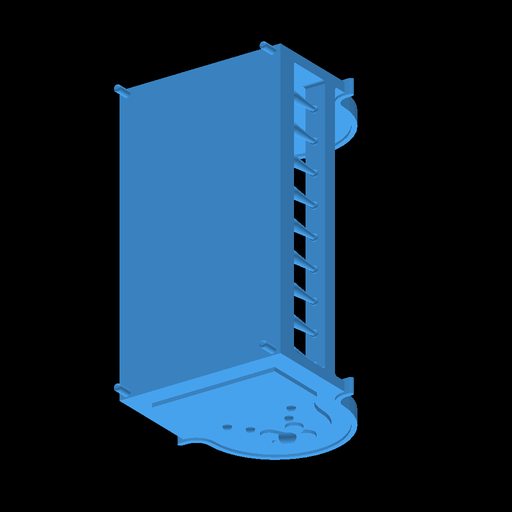
\includegraphics[width=.84\linewidth]{images/interior-target-rgb.png}
    \figlabel{\textbf{RGB}: границы и форма}
  \end{column}
  \begin{column}{.317\textwidth}
    \centering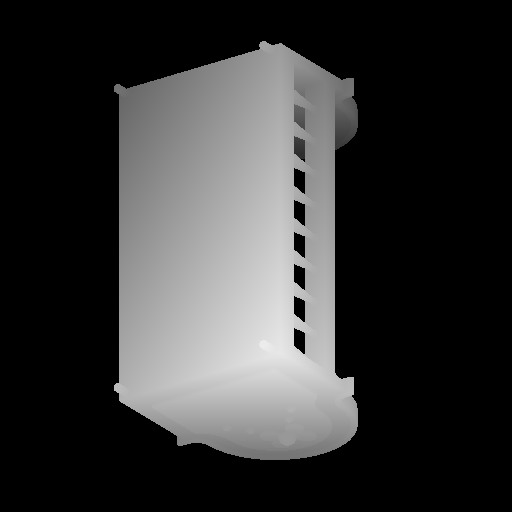
\includegraphics[width=.84\linewidth]{images/interior-target-depth.png}
    \figlabel{\textbf{Depth}: положение поверхности}
  \end{column}
  \begin{column}{.317\textwidth}
    \centering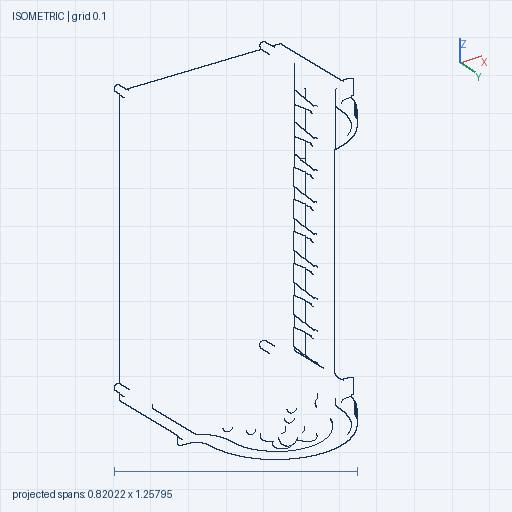
\includegraphics[width=.84\linewidth]{images/interior-target-blueprint.png}
    \figlabel{\textbf{Чертёж}: контуры, оси, сетка}
  \end{column}
\end{columns}
\medskip
{\smalltext
Шесть видов; исходник и CAD используют общие камеры и шкалу глубины.
Отдельный вызов составляет план геометрии перед генерацией кода.

\smallskip
Дополнительный контекст: габариты, девять сечений, объём и центр масс STL.
Каждый вызов анализа входит в стоимость.}
\source{Показан один из шести видов. Depth и чертёж получены из STL; произвольные фотографии
и внешние карты глубины в этот pipeline не подключены. Источник: vision.py, harness2.py.}
\end{frame}

% 5
\begin{frame}{Основная метрика и визуальная обратная связь}
\begin{columns}[T,onlytextwidth]
  \begin{column}{.58\textwidth}
    \textbf{Объёмный IoU}
    \[
      \IoU(M,\widehat M)=
      \frac{\operatorname{Vol}(M\cap\widehat M)}
           {\operatorname{Vol}(M\cup\widehat M)} .
    \]
    {\smalltext
    Булевы операции \texttt{manifold3d} над полными STL.
    Оценка доступна для корректных замкнутых объёмов.

    \smallskip
    Исходник центрируется; максимальный габарит равен 1.
    CAD оценивается без выравнивания и подгонки масштаба.

    \medskip
    \textbf{Вспомогательные показатели:}
    silhouette IoU, depth MAE на общих видимых пикселях,
    доля missing-граней поверхности.}
  \end{column}
  \begin{column}{.38\textwidth}
    \centering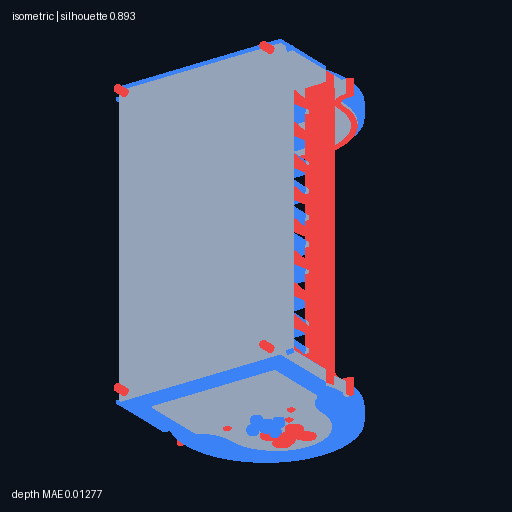
\includegraphics[width=.67\linewidth]{images/interior-difference.png}
    \figlabel{\textbf{Схема глубины}\\
      Красный: нет поверхности / дальше\\
      Синий: лишняя поверхность / ближе}
    \vspace{2mm}
    {\smalltext\alert{Метрики видов не заменяют объёмный IoU.}}
  \end{column}
\end{columns}
\source{Источник: geometry.py, vision.py. Missing считается по размеченным граням, не по объёму.
Удаляются только вырожденные грани; отверстия STL не заполняются.}
\end{frame}

% 6
\begin{frame}{Данные и протокол пилотных экспериментов}\relax
{\smalltext
\begin{tabular}{@{}p{.23\textwidth}p{.36\textwidth}p{.34\textwidth}@{}}
\toprule
\textbf{Набор} & \textbf{В манифесте} & \textbf{В экспериментах}\\
\midrule
DeepCAD & 10 dev + 100 test; seed 42 & 3 dev: оркестратор 1;\newline 1 dev: оркестратор 2\\
Interior300 & 300 STL: 240 IndoorCAD,\newline 60 Poly Haven; 118 объёмных & 1 объект: оркестратор 2;\newline локальный split \texttt{all}\\
\bottomrule
\end{tabular}}
\medskip
\begin{itemize}
  \item \texttt{openai/gpt-6-luna}; код: \texttt{medium}, анализ: \texttt{low}.
  \item Оркестратор 1: до пяти программ; второй: до двух
        программ и один анализ геометрии.
  \item Стоимость берётся из provider usage и включает все вызовы,
        в том числе неудачные ответы.
\end{itemize}
\source{SHA-256 входов и снимки manifest сохранены. DeepCAD: локальная STL-выборка,
не полный официальный benchmark. 182 модели Interior300 не имеют объёмного IoU.
Результаты ниже относятся к выбранным объектам; пакетная test-оценка здесь не выполнена.}
\end{frame}

% 7
\begin{frame}{DeepCAD: предварительное сравнение}\relax
{\small\textbf{Одна dev-деталь:} \texttt{274a034e5c4ac827} / \texttt{00189070.stl}}
\medskip
\begin{columns}[T,onlytextwidth]
  \begin{column}{.57\textwidth}
    {\smalltext
    \begin{tabular}{@{}lrr@{}}
    \toprule
      & \textbf{Орк. 1} & \textbf{Орк. 2}\\
    \midrule
    Лучший IoU & \ClassicIoU & \textbf{\DeepIoU}\\
    Валидные программы & 5/5 & 1/2\\
    Вызовы LLM & 5 & 3\\
    Все вызовы, USD & \ClassicCost & \DeepCost\\
    \bottomrule
    \end{tabular}

    \medskip
    Во втором режиме лучший CAD получен с первой программы.
    Следующий ответ не исполнился; лучший результат сохранён.

    \medskip
    \alert{Различаются визуальный контекст и бюджеты.
    Это пилот, а не контролируемая абляция.}}
  \end{column}
  \begin{column}{.39\textwidth}
    \begin{columns}[T,onlytextwidth]
      \begin{column}{.485\textwidth}
        
\includegraphics[width=\linewidth]{images/deepcad-target.png}
        \figlabel{Исходник}
      \end{column}
      \begin{column}{.485\textwidth}
        
\includegraphics[width=\linewidth]{images/deepcad-v2.png}
        \figlabel{CAD, орк. 2}
      \end{column}
    \end{columns}
    \vspace{3mm}
    {\smalltext Орк. 2: \DeepSeconds\,с;\newline
    пик RSS \DeepMemory\,МиБ;\newline
    цель IoU $0.95$ не достигнута.}
  \end{column}
\end{columns}
\source{Источник: run.json запусков 20261022T184742Z-b4c867e2 и 20261022T184705Z-7cef923e.
Для оркестратора 1 указаны затраты только этой детали, не всей очереди из трёх STL.}
\end{frame}

% 8
\begin{frame}{Interior300: исправление по обратной связи}\relax
{\small \textbf{Объект:} \texttt{indoorcad\_d8441ba72f8641} / \texttt{baby bed\_SLDPRT}}
\medskip
\begin{columns}[T,onlytextwidth]
  \begin{column}{.317\textwidth}
    \centering
\includegraphics[width=.79\linewidth]{images/interior-target-right.png}
    \figlabel{Исходный STL}
  \end{column}
  \begin{column}{.317\textwidth}
    \centering
\includegraphics[width=.79\linewidth]{images/interior-first-right.png}
    \figlabel{Программа 1: IoU \InteriorFirst}
  \end{column}
  \begin{column}{.317\textwidth}
    \centering
\includegraphics[width=.79\linewidth]{images/interior-second-right.png}
    \figlabel{Программа 2: IoU \textbf{\InteriorBest}}
  \end{column}
\end{columns}
\medskip
{\smalltext
\textbf{Две валидные программы; прирост IoU \InteriorGain.}
Агент изменил конструкцию по метрикам и схеме ошибок.
Численная оптимизация не использовалась.

\smallskip
Полный цикл: 3 вызова LLM; \$\InteriorCost;
\InteriorSeconds\,с; пик RSS \InteriorMemory\,МиБ.}
\source{Источник: run.json, код и STL запуска 20261022T185141Z-59366e3d.
Один объект, общий вид и координаты; вывод о всём наборе не делается.
Missing surface: 22.9\% → 51.5\%; прирост IoU не означает улучшения всех метрик.}
\end{frame}

% 9
\begin{frame}{Реализация и воспроизводимость}
\begin{columns}[T,onlytextwidth]
  \begin{column}{.52\textwidth}
    \textbf{Сохранение эксперимента}
    \begin{itemize}
      \item Снимок STL, SHA-256 и нормализация.
      \item Точные запросы, ответы, код, STEP/STL.
      \item IoU, метрики видов, usage и причины отказов.
      \item Checkpoint и повторное использование сохранённых ответов.
    \end{itemize}
  \end{column}
  \begin{column}{.44\textwidth}
    \textbf{Исполнение и наблюдение}
    \begin{itemize}
      \item Один тяжёлый worker; очередь.
      \item RSS worker и дочерних CAD-процессов: лимит 2048 МиБ.
      \item Streamlit: preview и выбранная итерация.
      \item Консоль проекта и журнал событий этапов.
    \end{itemize}
  \end{column}
\end{columns}
\medskip
{\smalltext
Оплаченный ответ сохраняется до разбора кода. При обрыве HTTP до сохранения
повторная оплата возможна. RSS проверяется опросом: краткий выход за лимит
между замерами возможен.}
\source{Источник: harness.py, harness\_worker.py, resources.py, harness\_ui.py и observability.py.
Метрики и SHA-256 источников этой презентации: evidence.json; описание протокола: README.md.}
\end{frame}

% 10
\begin{frame}{Выводы и проверка гипотезы}
\textbf{Получено}
\begin{itemize}
  \item Реализован цикл генерации, исполнения и оценки CAD с визуальной
        обратной связью и сохранением лучшего результата.
  \item Два пилота показывают работоспособность; на интерьерном объекте
        вторая программа повысила объёмный IoU.
\end{itemize}

\medskip
\textbf{Следующий эксперимент}
\begin{itemize}
  \item Зафиксировать общие ID, бюджеты и конфигурации моделей.
  \item Сравнить одну генерацию, независимые кандидаты и исправления.
  \item Разделить вклад измерений, анализа, depth и чертежа;
        оценить IoU, отказы, полную стоимость и время по доменам.
\end{itemize}
\medskip
\alert{Сравнение с Qwen / Opus и экономия API в 5--10 раз пока не доказаны.}
\source{Текущие результаты не устанавливают среднее качество на DeepCAD test / Interior300
и не доказывают перенос на сканы или фотографии. Подробности и источники: speaker-notes.md, references.bib.}
\end{frame}

\end{document}
